\model{Computer Hardware}

\begin{center}
% source: Parts of the Computer - Micron K-12 Educator Resources
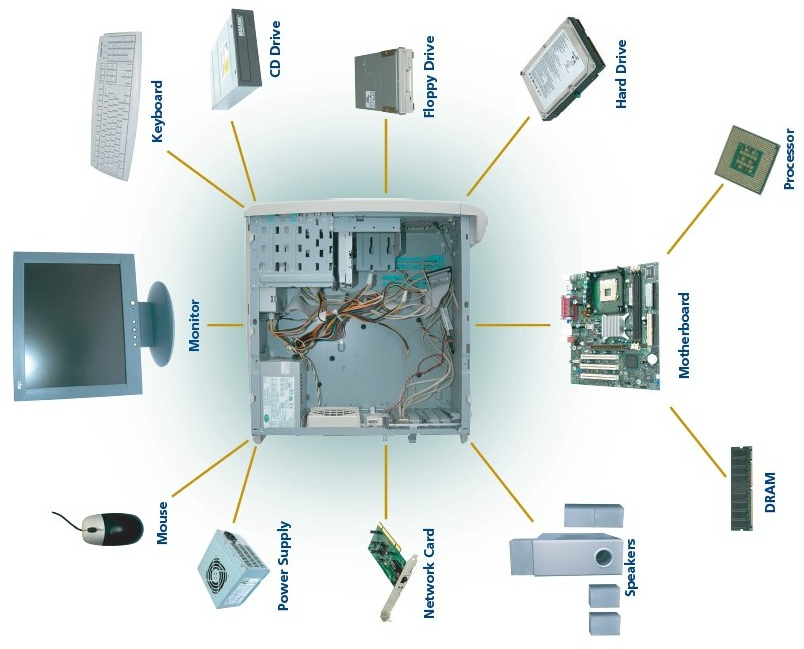
\includegraphics[height=3.65in]{CSP/computer1.png}
\end{center}


\quest{10 min}


\Q For each category, list examples of computer hardware and human anatomy.
(Keep it clean.)

\begin{table}[h!]
\begin{tabularx}{\linewidth}{l|X|X}
& Computer & Human \\
\hline
Input
  & \ans{keyboard, mouse, camera, mic}
  & \ans{eyes, ears, mouth, nose}
\\[4em]
\hline
Output
  & \ans{monitor, speakers, printer}
  & \ans{mouth, muscles, skin}
\\[4em]
\hline
Processing
  & \ans{CPU, network card, motherboard}
  & \ans{brain, heart, stomach}
\\[4em]
\hline
Storage
  & \ans{RAM, disk, flash}
  & \ans{fat cells, brain, bones}
\\[4em]
\end{tabularx}
\end{table}
